\documentclass{scrartcl}
\usepackage{fontspec} %connects to native fonts
\usepackage{amsmath}
\usepackage{mathtools}
\usepackage{cleveref}
\usepackage{pgfplots}
\usepackage{graphicx}
\usepackage{wrapfig}
\usepackage{fancyref}
\usepackage{amssymb}
\usepackage{subfig}
\usepackage{float}
\usepackage[justification=RaggedRight, singlelinecheck=false, font={footnotesize}]{caption}
\usepackage[portuguese]{babel}
\usepackage[title,titletoc,toc]{appendix}


\usepackage{lipsum}
\usepackage{blindtext}
\addtokomafont{sectioning}{\rmfamily}

\begin{document}
\pagenumbering{arabic}
\bibliographystyle{plain}
\title{
	\textnormal{
	\LARGE Universidade de Lisboa - Instituto Superior Técnico\\
	\Large Licenciatura em Engenharia Informática e de Computadores\\
	\Large Análise e Síntese de Algoritmos
\\}
	\LARGE2º Projeto
	\vspace{-1ex}
	}
\author{Gonçalo Marques,
	\texttt{84719}
	\and
	Manuel Sousa,
	\texttt{84740}
}
\date{	\vspace{-1ex}
		\vspace{-4ex}
	}
\maketitle

\section*{Introdução}
Com este projeto pretendemos apresentar uma solução eficiente para o problema enunciado, explicar a sua implementação e fazer uma análise teórica e experimental da complexidade temporal e espacial do mesmo.

\section*{Descrição do problema}
O problema consiste em calcular o custo mínimo de contruir um certo número de estradas e aeroportos entre várias cidades para que seja possível viajar para qualquer cidade, a partir de outra qualquer. Uma estrada liga duas cidades em ambos os sentidos. Cada cidade pode ter um aeroporto, a partir do qual tem acesso a todas as outras cidades que tenham aeroportos. Quer as estradas, quer os aeroportos têm um custo. Para além de calcular o custo mínimo de construir a rede de transportes, tem de ser indicado o número de estradas e aeroportos que compõem essa rede, tendo em atenção que se existirem várias soluções mínimas que têm o mesmo custo, então a solução aceite será a que tiver menos aeroportos. Se não for possível contruir uma rede mínima que inclua ligações entre todas as cidades, então os dados para construir a rede são insuficientes.

Ora este problema pode ser descrito como um problema num grafo não dirigido, pesado, em que:
\begin{itemize}
\setlength\itemsep{-0.5ex}
\item cada cidade é um nó
\item cada estrada ou aeroporto é uma aresta, e o seu custo, o peso dessa aresta
\end{itemize}

Assim, o problema descrito é equivalente ao de calcular num grafo não dirigido e pesado $G(V,E)$ (com $V = \#N$ e $E = \#A+\#R$ ou $E = \#R$, sendo $N$ o número de cidades, $A$ o número de cidades com aeroportos e $R$ o número de estradas existentes a ligar varias cidades), o custo total de uma árvore abrangente de menor custo , também conhecida em inglês como \textit{Minimum Spanning Tree} (MST). Temos de calcular também, o número de estradas e aeroportos que compõem essa rede de custo mínimo.

\section*{Algoritmo utilizado}
Tendo a solução do problema sido estudada nas aulas, foi utilizado o algoritmo de Prim para o cálculo do custo total da árvore abrangente de menor custo. \cite{prim} Para realizar uma solução bastante eficiente, contruímos uma Fibonacci Heap como fila de prioridades (\textit{min-priority queue}) para reduzir os tempos de acesso a estra estrutura executados pelo algoritmo. \cite{tarjan}

\section*{Estruturas utilizadas:}
\begin{itemize}
\setlength\itemsep{-0.5ex}
\item \textbf{G[$u$][i]} - O grafo $G$ foi representado como uma lista de adjacências (foi utilizado um std::vector (array dinâmica) em vez de std::list (lista duplamente ligada), pelo facto de a implementação do std::vector ser bastante mais eficiente que a de std::list \cite{ISOC++:2003}).
\item \textbf{visited[$u$]} - O nó $u$ foi visitado?
\item \textbf{taken[$u$]} - O nó $u$ existe na MST?
\item \textbf{pq} - Fibonnacci Heap utilizada pelo Prim
\end{itemize}
Todas estas estruturas (com exceção da Fibonnacci Heap) foram implementadas com o std::vector de C++ que tem tempo de inserção no fim $O(1+)$ e de acesso $O(1)$. Com tempo de inserção $O(1+)$ (constante amortizado), queremos dizer que para inserir $N$ elementos a complexidade de pior caso é $O(V)$, apesar da complexidade de pior caso de inserção de 1 elemento não ser $O(1)$ (de facto é também $O(V)$). \cite{ISOC++:2003}

\section*{Explicação do algoritmo}

Temos de considerar duas situações. A primeira situação consiste em ter em conta estradas e aeroportos na solução mais "barata". Para representar os aeroportos no grafo tem que se criar uma ligação lógica que tenha em conta as cidades com aeroportos e o custo de construir cada um deles. Para isso, cria-se um nó adicional no grafo chamado "Cidade Aérea", ao qual todas as cidades que têm aeroportos se ligam, através de arestas no grafo. Deste modo todas as cidades que possam ter um aeroporto ficam ligadas entre si, sendo o custo de um aeroporto registado em cada uma das arestas.

A segunda situação consiste em considerar apenas estradas. Neste caso ignoramos por completo os aeroportos (retirando-os do grafo), e calculamos o respetivo custo mínimo de uma possível rede. Por fim, a solução final será o menor custo das duas situações.

Antes de ter em conta cada umas das duas situações temos de nos preocupar com a conectividade do grafo. Se o grafo não for conexo então não é possível calcular uma rede que ligue todas as cidades, visto que há um conjunto de cidades que não terá ligações para pelo menos uma das outras (formando uma espécie de ilha). Para isso é executada uma pesquisa em profundidade com apenas uma chamada à função de DFSVisit num nó arbitrário (ao contrário de uma DFS completa que chama a função DFSVisit em todos os nós não visitados). Para cada nó visitado na DFS é guardada informação relativa ao seu estado de visita (vetor visited). Quando a pesquisa em profundidade terminar, percorremos de forma linear o nosso vetor visited por forma a encontrar um nó que não tenha sido visitado durante a pesquisa. Se isso acontecer então o nosso grafo não é conexo, visto que a partir de 1 nó, não foi possível visitar o grafo todo.

Para calcular o custo mínimo num grafo utilizamos o algoritmo de Prim que começa num nó inicial (por simplicidade começamos no nó 1) e marca o nó como visitado. De seguida o algoritmo escolhe a aresta cujo custo é mais pequeno (em caso de empate privilegia arestas que identificam estradas), dentro dos nós já visitados, e adiciona-a à MST. Sempre que o algoritmo escolhe uma aresta, marca o novo nó como visitado e passa a ter em conta as arestas desse nó. O algoritmo de Prim apenas escolhe arestas que tenham como extremidade um nó que ainda não tenha sido visitado (de forma a que a nova inserção nao forme um ciclo na MST).

Se os ambos grafos forem conexos, então escolhemos a solução mais "barata" das duas, e em caso de empate, aquela cujo número de aeroportos for menor.

\section*{Análise assintótica temporal teórica do algoritmo}

Para verificarmos a conectividade de um grafo no pior caso teremos $O(max(N-1,L))$ = $O(N+L)$ (caso geral) que equivale a visitar todos os nós do grafo, menos 1.

Para calcular a MST, teremos de correr o algoritmo de Prim. Dado que com uma Fibonacci Heap como fila de prioridades conseguimos tempos de inserção e de Decrease-Key de $O(1+)$ (constante amortizado). Para escolher e remover a aresta com o peso mais baixo temos $O(log(E)+) = O(log(V)+)$ (amortizado) visto que se $E = V^2$ temos $O(log(E)) = O(log(V^2)) = O(2Log(V)) = O(log(V))$.Concluímos então que a complexidade total do algoritmo de Prim com Fibonacci Heap como fila de prioridades será de $O(E + V log (V))$.

Podemos também considerar que teremos sempre complexidade de melhor e pior caso $O(E + V log (V))$ se um dos grafos contruídos numa das 2 situações (enunciadas na descrição do problema) for conexo. Se nenhum dos grafos for conexo, então a complexidade do algoritmo fica limitada ao tempo de construção do grafo que será de $O(V + E)$, visto que a verificação de conectividade de um grafo será sempre menor ou igual a $O(V + E)$.

\section*{Binary Heap V.s. Fibonacci Heap}

O uso de Fibonacci Heap como fila de prioridades trás claras vantagens de eficiência na resolução deste problema em comparação, por exemplo, com uma Binary Heap que tem tempo de inserção de $O(log(E)) = O(log(V))$, em contraste ao tempo $O(1+)$ (constante amortizada) da Fibonacci Heap. Portanto a complexidade final do algoritmo de Prim com Binary Heap será $O(Vlog(V) + Elog(V)) =  O(Elog(V))$, que é bastante pior (para grafos muito densos) considerando a complexidade de $O(E + V log(V))$ ($O(E)$ para grafos muito densos) do algoritmo de Prim com Fibonacci Heap.

Numa experiência com 50.000 cidades (nós) e uma soma de aeroportos com estradas de 8.050.000 (arestas), o algoritmo de Prim com Binary Heap como fila de prioridades precisou de 41,5 segundos de CPU para calcular a solução, e o mesmo algoritmo com Fibonacci Heap precisou de apenas 8,6 segundos.

Provamos assim que a utilização de uma Fibonacci Heap como fila de prioridades, torna a solução significativamente mais rápida em termos de eficiência.


\section*{Análise assintótica espacial}
Como se verifica pelas estruturas utilizadas, o algoritmo utiliza duas estruturas com $N$ booleanos (visited e taken), e uma estrutura com $N$ vetores, mas com o total de $L$ arestas (representadas com std::pair, sendo o pair <custo, vértice de ligação>) no seu interior. Como é tudo guardado sobre variáveis locais podemos concluir que a memória de stack tem complexidade de pior caso $O(V+E)$, que é o custo de representar o grafo.


\section*{Análise assintótica temporal experimental do algoritmo}
\begin{wrapfigure}{r}{0.5\textwidth}
	\centering
	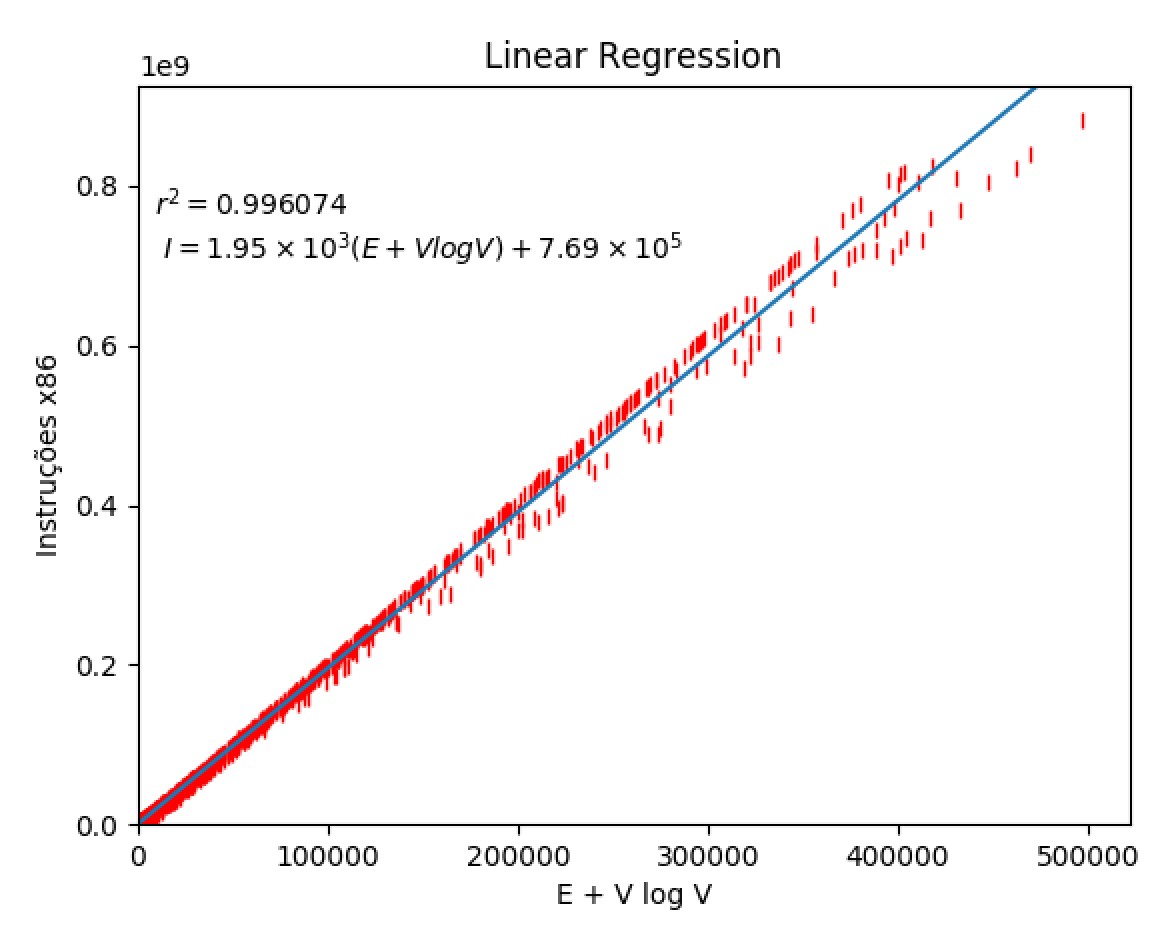
\includegraphics[width=0.4\textwidth]{img/analise.png}
	\caption{Análise experimental com parâmetros $2 \le N \le 1000 $ (1000 riscos)}
	\label{fig:analexp}
\end{wrapfigure}
Para se realizar a análise experimental temporal do algoritmo, foi utilizada a aproximação que cada instrução de C corresponde em média a um número fixo de instruções de CPU. Assim, em primeiro lugar procedeu-se à geração de $K$ diferentes casos de teste aleatórios para soluções não Insuficientes (para cada caso foi escolhido aleatoriamente um $V$ e um $E\le \frac{V^2}{2}$). De seguida, para cada caso de teste foi utilizada a ferramenta perf para contar o número de instruções de CPU utilizadas em modo utilizador durante a execução do programa - $I$. Por fim, fez-se o plot do gráfico de $I$ em função da complexidade do algoritmo de Prim com Fibanacci Heap, ou seja, $E + V log (V)$. Obteve-se assim os resultados da Figura \ref{fig:analexp}.\par
Sendo o coeficiente de correlação linear muito próximo de 1, a análise experimental comprova o resultado teórico esperado.

\bibliography{ref}

\end{document}


